\documentclass{beamer}

\setbeamercolor{palette primary}{bg=black,fg=white}
\setbeamercolor{palette secondary}{bg=black,fg=white}
\setbeamercolor{palette tertiary}{bg=black,fg=black}
\setbeamercolor{palette quaternary}{bg=black,fg=white}
\setbeamercolor{structure}{fg=black} % itemize, enumerate, etc
\setbeamercolor{section in toc}{fg=black} % TOC sections

\beamertemplatenavigationsymbolsempty
\usefonttheme[onlymath]{serif}

\usepackage{graphicx}

\newcommand{\nn}{\nonumber\\}
\renewcommand{\P}{\mathcal{P}}
\renewcommand{\L}{\mathcal{L}}
\newcommand{\M}[1]{\mathcal{M}_{\rm max}^{#1}}
\newcommand{\I}[1]{{I_{#1}}}
\newcommand{\J}[1]{{J_{#1}}}

\title{Multipole Mermin-Wagner Constraints}
\subtitle{}
\author{Charles Stahl}
\institute{University of Colorado \\ Department of Physics}
\date{February 18, 2022}

\AtBeginSection
{
  \begin{frame}
    \frametitle{Outline}
    \tableofcontents[currentsection]
  \end{frame}
}

\begin{document}

\frame{\titlepage}

%\begin{frame}{Outline}
%Ordinary Mermin-Wagner theorem\\\
%
%Multipole symmetries\\\
%
%Multipole field theories and Mermin-Wagner\\\
%
%\hrule
%\vspace{6pt}
%
%Mermin-Wagner for partial breaking of multipole symmetries
%\end{frame} 

\section{Ordinary Mermin-Wagner theorem}

\begin{frame}{Mermin-Wagner theorem}
Consider a system with an internal $U(1)$ symmetry\\\

Assume the symmetry is broken $\rightarrow$ Goldstone boson
\begin{align*}
\L = (\partial_t \phi)^2 + (\partial_i \phi)^2
\end{align*}
Correlation functions go as
\begin{align*}
\langle \phi(x,t) \phi(0,0) \rangle &= \int \frac{d\omega dk \, k^{d-1}}{\omega^2+ k^2}\\ 
&= \int \frac{dk}{k} k^{d-1},
\end{align*}
which diverges (in the IR) when $d\le 1$
\end{frame}

\begin{frame}{Interpretation}
When the correlation function does not diverge ($d>1$), there can be a phase distinguished by symmetry properties\\\

At the critical dimension ($d=1$), there can still be a phase distinguished by a non-vanishing compressibility

\setlength{\leftskip}{1cm}

Luttinger liquid

Quasi-long-range order
\end{frame}

\section{Multipole symmetries}

\begin{frame}{Multipole symmetries}
Recall that an ordinary symmetry acts as $\phi(x) \rightarrow \phi(x) + c$\\\

Gauge ``symmetries" are not physical symmetries\\\

Generalize to $\phi(x) \rightarrow \phi(x) + P(x)$

\setlength{\leftskip}{1cm}

$P(x) = a_ix^i + b$, $c(x^2+1)$, etc.\\\

\setlength{\leftskip}{0cm}

Gauging these symmetries can lead to fractons [Pretko 2018]
\end{frame}

\begin{frame}{Multipole groups}
Choose an internal group $G_{\rm int}$ and a set of polynomials\\\

The internal group has to be Abelian [Glorioso et. al. 2020], stick with $G_{\rm int}=U(1)$\\\

There is a generator corresponding to each polynomial [Gromov 2019]

\setlength{\leftskip}{1cm}

$\mathcal{P}_0, \P_1^i, \P_2^{ij}$, etc.\\\

$\exp(c \P_0) \phi(x) = \phi(x) +c$\\\

$\exp (a_{ij} \P_2^{ij}) \phi(x) = \phi(x) + a_{ij} x^i x^j$\\

\setlength{\leftskip}{0cm}

\small (restriction to monomials makes indices simpler)
\end{frame}

\begin{frame}{Multipole groups}
Generators might not commute with space symmetries [Gromov 2019]
\begin{align*}
[T_j, \P_a^{i_1\dots i_a}] &= \delta^{i_m}_j \P_{a-1} ^{i_1\dots i_{m-1}i_{m+1}\dots i_a}\\
[R_{jk}, \P^{i_1\dots i_a}_a] &= \delta_{[j}^{(i_1} \P^{k]i_2)\dots i_a}_a
\end{align*}

For example, $[T_1,\P_1^1] = \P_0$ and $[R_{12}, \P_1^1] = \P_1^2$\\\

Include all resulting polynomials, or exclude some translations or rotations
\end{frame}

\begin{frame}{Maximal multipole group}
$\M{a}$ contains all polynomials of degree $<a$

Note: this is NOT the definition in the literature, but it makes formulas nicer\\\

Any multipole group is therefore a subgroup of $\M{a}$ for some $a$\\\

Also contains all translations and rotations\\\

$\M{1}$ is ordinary $U(1)$, $\M{0}$ is the trivial group
\end{frame}

\section{Multipole field theories and Mermin-Wagner}

\begin{frame}{Multipole-invariant field theories}
Example: $\mathcal{L} = (\partial_t \phi)^2 + g (\partial_i \partial_j \phi)^2$ is invariant under $\M{2}$\\\

For a generic multipole group, it is not possible to find such a theory [Gromov 2019]\\\

Interesting examples do exist, and can lead to fracton phases after gauging [Pretko 2018; Gromov 2019]\\\

A special example leads to Haah's code [Bulmash, Barkeshli 2018]
\end{frame}

\begin{frame}{Multipole-invariant field theories}
Stick with rotationally invariant theory
\begin{align*}
\L &= (\partial_t \phi)^2 + g(\partial_{I_a} \phi)^2,
\end{align*}
where $I_a = i_1 \dots i_a$ is a multi-index and 
\begin{align*}
\partial_{I_a} = \partial_{i_1}\dots \partial_{i_a}
\end{align*}
This is invariant under $\M{a}$\\\

Interesting things to say about total derivatives and rotational invariance...
\end{frame}

\begin{frame}{Mermin-Wagner for multipole theories}
$\L = (\partial_t \phi)^2 + g (\partial_{I_a} \phi)^2$\\\

Assume the $\phi$ field exists. Is long-range order possible?
\begin{align*}
\left\langle \phi(x,t) \phi(0) \right\rangle &\sim \int \frac{d\omega dk\, k^{d-1}}{\omega^2 + k^{2a}}\\
&= \int \frac{dk}{k} k^{d-a}
\end{align*}

IR divergence for $d\le a$ [Griffin 2015]\\\

Critical dimension at $T=0$ is $d_{\rm c} = a$
\end{frame}

\begin{frame}{Mermin-Wagner for multipole theories}
What other possibilities are there?\\\

Non-maximal groups, eg. Haah group\\\

Partial breaking from $\M{a} \rightarrow \M{c}$\\\

Combine both?
\end{frame}

\section{Mermin-Wagner for partial breaking of multipole symmetries}

\begin{frame}{Mermin-Wagner for partial breaking, I}
Naive method to break from $\M{a}$ to $\M{c}$ with $c<a$\\\

Define field $\phi_{i_1\dots i_c} = \phi_\I{c}$

\setlength{\leftskip}{1cm}

$\exp(\beta_{I_b} \P_b^{I_b})\phi_{J_{c}}(x) = \phi_\J{c} + \beta_{\J{c}\I{b-c}} x^\I{b-c}$

Invariant under polynomials of degree $<c$

$\phi_\I{c}$ develops LRO: $\M{a} \rightarrow \M{c}$\\\

\setlength{\leftskip}{0cm}

Example: $\phi_i$ would break the dipole group $\M{2}$ to the monopole group $\M{1}$\\\

[CNS, Lake, Nandkishore]
\end{frame}

\begin{frame}{Mermin-Wagner for partial breaking, I}
Naive result: can $\phi_\I{c}$ develop LRO?\\\

Consider $\L = (\partial_t \phi_\I{c})^2 + (\partial_\J{a-c} \phi_\I{c})^2$. Then
\begin{align*}
\left \langle \phi_\I{c} (x,t) \phi_\I{c} (0) \right \rangle &\sim \int \frac{d\omega dk\, k^{d-1}}{\omega^2 + k^{2a-2c}}\\
&= \int \frac{dk}{k} k^{d-a+c}
\end{align*}
It looks like the critical dimension should be $d_{\rm c} = a-c$\dots
\end{frame}

\begin{frame}{Mermin-Wagner for partial breaking, II}
The operator $\partial_\I{c-b} \phi_\J{b}$ is breaks $\M{a} \rightarrow \M{c}$\\\

Let's look at the theory $\L = (\partial_t \phi_\J{b})^2 + (\partial_\I{a-b} \phi_\J{b})^2$

\setlength{\leftskip}{1cm}

First $b$ compressibilities are all 0 $\rightarrow$ specifies theory

$\kappa_e \equiv \frac{d \langle n_e^\I{e} \rangle}{d \mu_e^\I{e}}=0$ for $e\le b$\\\

\setlength{\leftskip}{0cm}

Now the correlation function becomes
\begin{align*}
\langle \partial_\I{c-b} \phi_\J{b} (x,t) \partial_\I{c-b} \phi_\J{b} (0,0) \rangle &= \int \frac{d\omega dk\,k^{d-1}\, k^{2(c-b)}}{ \omega^2 + k^{2(a-b)}}\\
&= \int \frac{dk}{k}k^{d-a-b+2c}
\end{align*}
and $\partial_\I{c-b} \phi_\J{b}$ can only order if $d \ge a+b-2c$
\end{frame}

\begin{frame}{Interpreting the critical dimension}
$a$ and $b$ define the theory, $c$ defines the preserved subgroup\\\

At fixed $a,b,c$

\setlength{\leftskip}{1cm}

In this theory, $\M{c+1}$ can only be broken if $d > a+b-2c$

Doesn't tell you what the preserved subgroup actually is\\\

\setlength{\leftskip}{0cm}

At fixed $a,b,d$: What is the preserved subgroup?

\setlength{\leftskip}{1cm}

$\M{c}$ is broken for $c > (a+b-d)/2$

Preserved subgroup is $\M{\lfloor (a+b-d)/2 \rfloor} $\\\

\setlength{\leftskip}{0cm}

At fixed $a,c$: When is this SSB possible?

\setlength{\leftskip}{1cm}

Critical dimension is $d = \min_b a+b-2c = a-2c$

Symmetry breaking is possible at $d=1$!
\end{frame}

\begin{frame}{Example: dipolar Bose-Hubbard model}
Bose-Hubbard model with dipole constraint imposed
\begin{align*}
H = -t \sum_{i,\mu,\nu} b^\dagger_i b_{i+\mu} b^\dagger_{i+\mu+\nu} b_{i+\nu} -\mu \sum_i n_i + \frac{U}{2} n_i(n_i-1)
\end{align*}
\begin{figure}
	\centering
	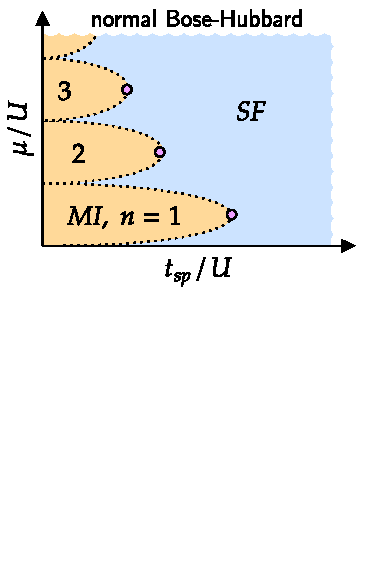
\includegraphics[scale=.8]{bhm}
	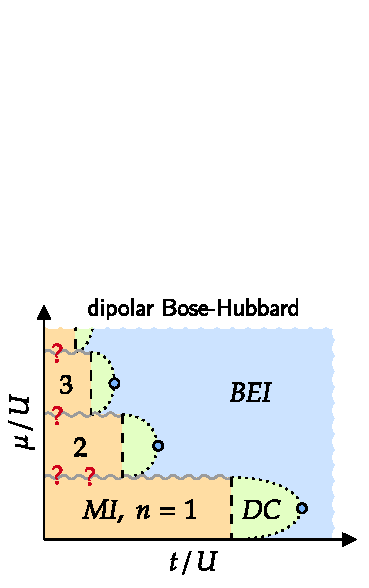
\includegraphics[scale=.8]{dbhm}
\end{figure}
[Lake, Hermele, Senthil]
\end{frame}

\begin{frame}[t]{Example: dipolar Bose-Hubbard model}
\begin{figure}
	\centering
	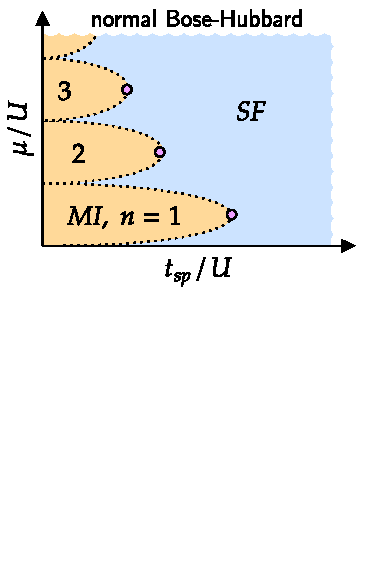
\includegraphics[scale=.8]{bhm}
	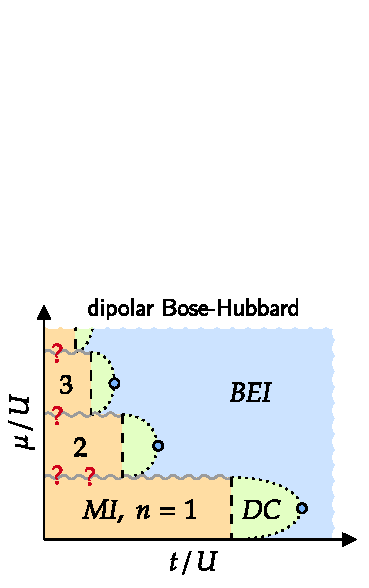
\includegraphics[scale=.8]{dbhm}
\end{figure}
Dipole Condensate: \hspace{.2cm} $(\partial_t \phi_i)^2 + (\partial_j \phi_i)^2 \quad (b=1)$\\\

Bose-Einstein Insulator: $(\partial_t \phi)^2 + (\partial_j \phi)^2 \quad (b=0)$
\end{frame}

\begin{frame}[t]{Example: dipolar Bose-Hubbard model}
\begin{figure}
	\centering
	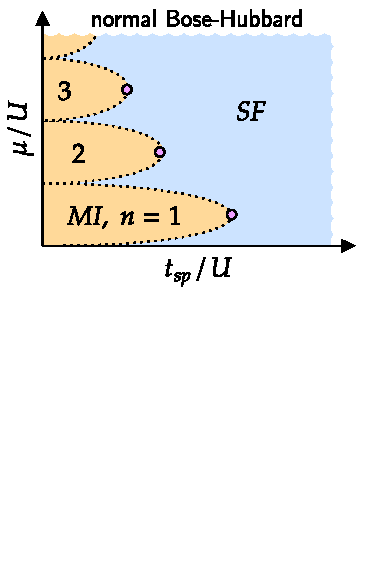
\includegraphics[scale=.8]{bhm}
	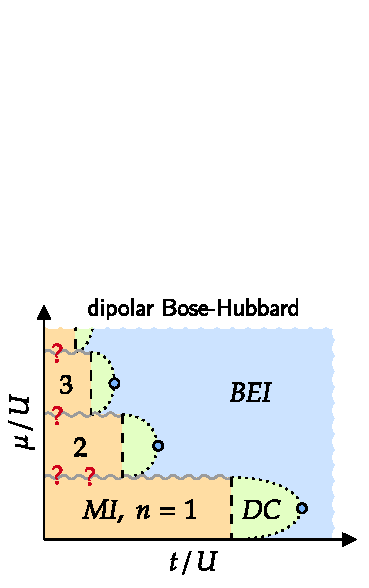
\includegraphics[scale=.8]{dbhm}
\end{figure}
Normal Bose-Hubard model

\setlength{\leftskip}{1cm}

$d\ge 2$: SF has SSB $\M{1} \rightarrow \M{0}$

$d=1$: SF has no SSB, instead has QLRO
\end{frame}

\begin{frame}[t]{Example: dipolar Bose-Hubbard model}
\begin{figure}
	\centering
	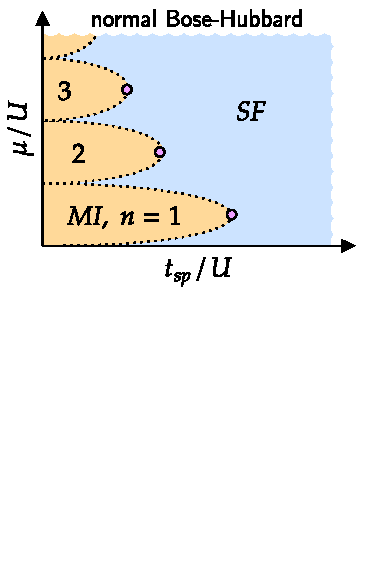
\includegraphics[scale=.8]{bhm}
	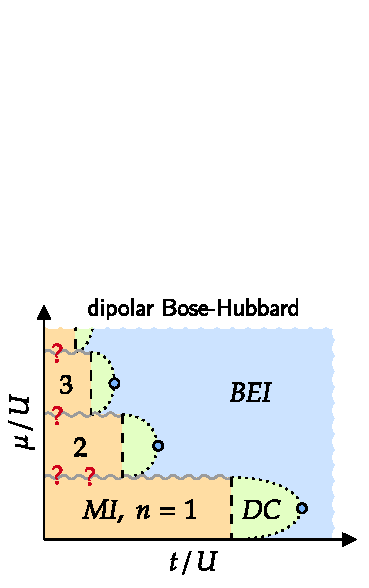
\includegraphics[scale=.8]{dbhm}
\end{figure}
Dipolar Bose-Hubard model

\setlength{\leftskip}{1cm}

$d\ge 3$: BEI:$\M{2} \rightarrow \M{0}$, DC: $\M{2} \rightarrow \M{1}$

$d=2$: BEI:$\M{2} \rightarrow \M{1}$, DC: $\M{2} \rightarrow \M{1}$

$d=1$: BEI:$\M{2} \rightarrow \M{1}$, DC: $\M{2} \rightarrow \M{2}$
\end{frame}

\end{document}